\chapter{Program OSM\_Navigation}
\paragraph{}
Aplikáciu bola vyvíjaná v jazyku C++ s knižnicami Qt. Prečo práve Qt? Qt je jednoduché rozhranie a programátori ho majú radi. Vývoj tejto aplikácie prebiehal pod operačným systémom Linux a vo vývojovom prostredí Qt Creator. Dokumentácia bola generovaná pomocou aplikácie DoxyGen z komentárov v zdrojovom kóde aplikácie. 

Program bol vyvíjaný za účelom vizualizácie dát z gps prístrojov. Dáta sú interpretované na voľne dostupných OpenStreetMap mapách. Program môžme používať ako s gps prístrojom tak aj bez neho (zobrazovanie trás a bodov). 

Základ programu bol použitý z grafických vzorov knižnice Qt graphics-dojo. Viac o grafických vzoroch Qt Graphics Dojo nájdeme na stránke: \url{http://labs.trolltech.com/page/Graphics/About/Dojo}

\section{Výber programovacieho jazyka a vývojového\\ prostredia}
\paragraph{}Pri výbere programovacieho jazyka sme kládli dôraz hlavne na
jednoduchosť práce s obrázkami a mapovým zobrazením. Pri rozhodovaní boli
zvažované tieto prvky:
\begin{enumerate}
\item vhodné vzory pre danú prácu
\item množstvo dostupných knižníc na spracovanie dát
\item detailnosť popisu jednotlivých knižníc
\end{enumerate}
\paragraph{}
Pri výbere boli hlavnými konkurentmi programovacie jazyky C++, Java a Python.
Pri jazyku C++ je dostupné vývojové prostredie QT ktoré je multiplatformové.
Java je tiež vhodným konkurentom vzhľadom na vyspelosť vývojového prostredia. V
jazyku Python v spojení s Qt knižnicami vzniklo tzv. PyQt s ktorým je možné
pracovať vo vývojovom prostredí Eric4. 

Na vývoj softvéru v jazyku Qt môžeme mať viacero dôvodov. Toto prostredie nám ponúka kompletnú sadu nástrojov ako vývoj GUI, programovanie až po preklad aplikácie do viacerých jazykov. Samotný C++ jazyk v spojení z Qt knižnicami sa javí ako výkonnejší oproti jazyku Python v spojení s PyQt. Pri vykresľovaní dát tento jav môže značne ovplyvniť naše rozhodnutie.

Qt knižnica je rozsiahla a obsahuje všetky potrebné prvky pri vývoji softvéru. Aké nástroje na tvorbu Qt poskytuje môžeme vidieť aj vo vzorových príkladoch ktorých je veľké množstvo.\\


\paragraph{Qt} je multiplatformový\footnote{\textbf{multiplatformový} - softvér podporujúci rôzne platformy(Linux, Windows, MAC OS)} framework\footnote{\textbf{framework} - prostredie, v ktorom je organizovaná a napísaná ďalšia aplikácia, no je napísaná v tom istom jazyku} vytvorený na vývoj aplikácií.\\

\textbf{Vývojové prostredie sa skladá z viacerých prostriedkov a to:}
\begin{list}{•}
\item Qt Creator - hlavný vývojový nástroj
\item
\item Qt Designer - nástroj na grafické spracovanie GUI
\item Qt Linguist - vytvára podporu pre viacjazyčné aplikácie, vytváranie prekladov
\item Qt Assistant - dokumentácia pre knižnicu QT 
\end{list}

\subsection{Qt Creator}
\paragraph{} Nástroj určený pre vývoj aplikácií. 
Pri kompilácii sa zobrazuje výstup kompilácie. Počas behu aplikácie môžme vidieť výpisy priamo v prostredí.\\
Pri kompilácii si môžeme vybrať či budeme vytvárať debug mód, alebo konečnú
verziu programu. V samotnom prostredí je možnosť program debuggovať.

\section{Správa závislosti programu}
\paragraph{}
Tento nástroj umožňuje vytvorenie Makefile súboru, ktorý je potrebný pri
kompilácii väčšieho programu. Nástroj funguje bez rozdielu softvérovej platformy.
Kompilátor vyvára samotný Makefile súbor podľa toho v akej platforme sa nachádzame pretože pre samotnú platformu kompilátor ukladá konštanty ktoré sú v každej platforme špecifické. Veľkou výhodou tohto nástoja je že nám stačí vedieť malé množstvo informácií ku kompilácii samotného programu.

Projekt bol vytvorený vo vývojom prostredí Qt Creator a toto prostredie si od začiatku generuje projektový súbor (.pro) tento súbor aj automaticky dopĺňa podľa toho či pridávame ďalšie hlavičkové a zdrojové súbory.
\begin{flushleft}
Na vytvorenie závislostí programu nám stačí zadať príkaz:
\begin{verbatim}
  qmake-qt4 OSM_Navigaton.pro
\end{verbatim}
\end{flushleft}

Pri vytváraní Makefile súboru v prostredí Qt Creator sa pridávajú ďalšie časti do príkazu podľa toho či je samotný program kompilovaný v debug verzii alebo release.

Po vytvorení Makefile súboru stačí program skompilovať príkazom make. Príkaz make môžme použiť s rôznymi príponami, podľa toho čo chceme vykonať, čo zobraziť. 
\begin{flushleft}
\textbf{Príklad príkazu:}
\begin{verbatim}
  make -w
\end{verbatim}
\end{flushleft}

Musíme nachádzať v priečinku v ktorom je vytvorený súbor Makefile. príkaz si ho vie automaticky nájsť.
Jednou z používaných prípon je aj \textbf{-f [názov súboru]}(. Pri kompilácii väčšieho programu na počítači s viacerými jadrami je vhodné použiť príponu \textbf{-j [počet jadier na ktorých chceme kompilovať program]}

\section{Jazykové formáty programu}
\paragraph{}
Balík Qt podporuje multijazyčné aplikácie. V aplikácii bola snaha o dodržanie základných pravidiel pre vytvorenie multijazyčnej aplikácie. Ako základný jazyk každej aplikácie sa zvyčajne používa angličtina v tejto aplikácii je to podobne. Viditeľné súčasti ako tlačidlá a ponuky sú v anglickom jazyku. K tomu aby sme mohli preložiť čitateľné prvky na mape, je potrebné zapisovať ich názvy v kóde pomocou funkcie tr("text"), táto funkcia je statickou metódou všetkých grafických objektov v knižnici Qt.
\begin{flushleft}
\textbf{Príklad použitia:}
\begin{verbatim}
  QPushButton *home = new QPushButton(tr("Ž&ilina")); 
\end{verbatim}
\end{flushleft}

Použitím funkcie \textit{tr} budé zaistená možnosť pre multijazyčnosť aplikácie.\\\\
Pre nastavenie programu potrebujeme urobiť nasledujúce štyri kroky:
\begin{enumerate}
\item inicializovať preklady
\item pridať do projektového programu preklady
\item vytvoriť prekladový súbor
\item po úprave aktualizovať projektový súbor
\end{enumerate}
Po splnení krokov bude aplikácia automaticky načítavať domáci jazyk nastavený v operačnom systéme.
\begin{flushleft}
\textbf{Inicializácia prekladov:}
\begin{verbatim}
  QApplication app(argc, argv);
  QTranslator appTranslator;
  appTranslator.load(QString("OSM_Nav_") +QLocale::system().name());
  app.installTranslator(&appTranslator);
  app.setApplicationName("OSM_Navigation");

  return app.exec();
\end{verbatim} 
\end{flushleft}


Kód je potrebné vložiť do hlavnej časti programu pred spustením aplikácie, tú je ale potrebné kompilovať po vykonaní ďalších troch spomínaných krokov.
\begin{flushleft}
\textbf{Pridanie prekladov do projektového súboru:}
\begin{verbatim}
  TRANSLATIONS += OSM_Nav_en.ts
\end{verbatim} 

\textbf{Prekladový súbor vytvoríme zadaním príkazu do shellu\footnote{\textbf{shell} - príkazový riadok v Linuxe}:}
\begin{verbatim}
  lupdate OSM_Navigation.pro
\end{verbatim} 
\end{flushleft}

Tento príkaz musíme opakovať po každom pridaní súčastí do programu ktoré sú používateľovi viditeľné a bude ich potrebné prekladať do iného jazyka.
\begin{flushleft}
\textbf{Pri každej zmene v prekladovom súbore je potrebné vykonať príkaz:}
\begin{verbatim}
  lrelease OSM_Navigation.pro
\end{verbatim} 
\end{flushleft}

Samotná aplikácia pri inicializácii kontroluje či je domovský jazyk vytvorený a ak nie je tak inicializuje základný jazyk čo je v našom prípade angličtina.

\section{Aplikačná a dátová vrstva programu}
Aplikačná časť vytvára tzv. jadro programu, v ktorom prebiehajú všetky dôležité výpočty, potrebné pre neskoršie vykresľovanie. 
\subsection{Sťahovanie častí mapy}
\paragraph{}
Mapy program sťahuje len ak sme ešte na danej pozícii neboli, ak sa tak stalo tak mapy má už program stiahnuté na disku. Mapa je rozdelená na malé časti o konštantnej veľkosti v pixloch (v našom prípade je to 256*256 bodov). Z toho vyplýva že čím je priblíženie väčšie tým potrebujeme viac obrázkov na pokrytie celej mapy. Na prístup k internetovej adrese sme použili nasledujúcu knižnicu:
\paragraph{QUrl}
Knižnica umožňuje komunikáciu s akoukoľvek url adresou. 
v našom prípade sme ju používali v tomto tvare:
\begin{verbatim}
  QString path = "http://tile.openstreetmap.org/%1/%2/%3.png";
  m_url = QUrl(path.arg(zoom).arg(grab.x()).arg(grab.y())); 
\end{verbatim}

Argumenty do tejto adresy sú vypočítavané a pridávané podľa zemepisných súradníc na ktorých sa nachádzame.
Trieda QUrl sa používa v triede QNetworkAccessManager ktorá si dané obrázky ukladá do vopred vyhradenej pamäte.
Postupne sa kontroluje každá časť mapy a ak sa hľadaná mapa na disku nenachádza, tak sa program pokúša danú časť stiahnuť pomocou spomínaných tried. Po kontrole úspešnosti stiahnutia konkrétnej časti mapy program obrázok uloží na disku. Pomocou tejto triedy vieme načítavať dáta do triedy QHash. 
\paragraph{QHash} je trieda na hešovanie\footnote{\textbf{Hešovacia funkcia} - funkcia, ktorá prevádza vstupný reťazec do výstupného pomocou predpísaného kódu. Reťazec označujeme ako heš (angl. hash) a jeho dĺžka je závislá od zvolenej funkcie a musí mať fixnú dĺžku.} dát v našom prípade hešovanie obrázkov. K tejto triede je potrebné pripraviť hešovaciu funkciu pomocou ktorej sú dáta rozoznávané.
V tomto programe bola použitá táto hešovacia funkcia:
\begin{verbatim}
  uint qHash(const QPoint& p){
     return p.x() * 17 ^ p.y();
  }
\end{verbatim}

Ako kľúč v tejto funkcii bol argument bod(x,y) a pomocou tohto kľúča sa počas behu programu vyhľadávajú konkrétne časti mapy.

\subsection{Načítanie dát zo súboru}
\paragraph{}
Načítanie dát zo súboru prebieha vo formáte GPX, ak máme vstupné dáta v inom formáte je možné pomocou programu gpsbabel, ku ktorému existuje GUI aplikácia \textbf(Gebabbel). Vďaka tejto aplikácii môžeme dáta konvertovať do potrebného formátu a následne použiť v programe na vykreslenie dát.\\ 
Na načítavanie dát v programe je vytvorená trieda Tracks. V triede prebieha rozdelenie dát do jednotlivých zložiek, t.j. tratí a zaujímavých bodov(waypointov). Na čítanie z GPX súboru existuje v Qt modul QtXml. V tomto module sa nachádzajú všetky triedy potrebné na čítanie, zápis aj vytváranie XML súborov. Dát z trás je vo všeobecnosti oveľa väčšie množstvo ako zaujímavých bodov.  

Vzhľadom na to že v tomto programe boli využívané hlavne triedy z knižnice Qt, nebolo to inak ani pri načítavaní súboru. 
Pri čítaní bola použitá trieda \textbf{QFile} pomocou ktorej sa pracuje zo súbormi. Pri výbere cieľového súboru sme použili triedu \textbf{QFileChooser} v ktorej sa dá jednoducho nastaviť filter na konkrétny typ súboru (v našom prípade *.gpx). Pred začatím čítania zo súboru sa súbor otvorí na čítanie ako textový. \\
Pri rozdeľovaní súboru na jednotlivé časti boli potrebné nasledujúce triedy:
\paragraph{QXmlStreamReader}
Trieda do ktorej sa načítali dáta zo súboru. V triede je možné jednoducho čítať XML tagy a preto bola použitá. Pri rozdeľovaní dát postupne kontrolujeme meno konkrétneho tagu a podľa toho sa rozhodujeme čo ďalej urobiť. 
\paragraph{QXmlStreamAttributes}
Gps dáta sú uložené ako atribúty a preto je použitá táto trieda. Trieda vytvára z konkrétnych atribútov vhodné dáta na spracovanie. V našom prípade sú to zemepisné súradnice potrebné na vykreslenie trás a zaujímavých bodov. Tieto body je vhodné ukladať s použitím triedy QPointF, ktorá reprezentuje triedu s bodmi x,y s dátovým typom reálneho čísla. V Qt moduloch existuje trieda QVector ktorá reprezentuje dynamické pole. Túto triedu bolo vhodné využiť na vytvorenie jednotlivých trás a tiež zaujímavých bodov. Keďže trás býva v jednom súbore viacej tak ako riešenie boli vybrané kontrolné body pomocou ktorých sa trasy neskôr rozdelia na jednotlivé časti. 
Zoznam trás je tak reprezentovaný triedou \textit{QVector<QPointF>} a to preto lebo samotné trasy je nutné uchovať vo forme zemepisných súradníc počas celého ich životného cyklu v aplikácii.

\subsection{Prepočítavanie dát k zobrazeniu trasy}
\paragraph{}
Zobrazovanie dát prebieha paralelne s vykresľovaním mapy. Súbor a samotné rozdelenie dát na trasy a zaujímavé body prebehne osobitne a dáta vstupujú k vykresleniu ako návratová hodnota z triedy Tracks, funkcie open.\\
Dáta, ako už bolo spomínané sú vo formáte zemepisných súradníc a v tejto forme ich dostáva trieda \textbf{LightMaps}, v tejto triede nastane prepočet jednotlivých súradníc do bodov na mape. Trieda oddeľuje výpočty od ich vykreslenia a to takým spôsobom, že po prepočte posiela tieto dáta triede \textit{SlippyMap}. Pri posielaní dát, týkajúcich sa zaujímavých bodov nie sú dáta v zložitej triede ich štruktúra sa mení z reálnych hodnôt do celých čísel typu \textit{int} a to takýmto spôsobom:\\

\begin{flushleft}
\textbf{Kód v programe:}
\begin{verbatim}
  QVector<QPoint> waypoints;
  QPoint p;                

  for(int i=0;i < waypointCoor.size();i++){
      p = getPixelFROMlatitude(waypointCoor.at(i));
      if(rangeIn(p,0)){
         waypoints.append(p);                
      }
  }
  m_normalMap->setWpt(waypoints);
\end{verbatim}
\end{flushleft}

V tejto funkcii získavame zo vstupných GPS súradníc ich hodnoty v pixloch. Funkcia \textit{rangeIn} vracia hodnotu true, ak sa daný bod nachádza na viditeľnej časti mapy. Výhodou takejto kontroly je rýchlejšie vykreslenie dát pretože program sa nesnaží vykresliť dáta mimo viditeľnej plochy. Pri vykresľovaní trás je problematika omnoho väčšia a to preto, lebo ak existuje trasa ktorá má väčšie množstvo bodov (trasa nasnímaná pri chodení z jedného miesta na druhé a naspäť) musíme vykresliť nie jednu súvislú čiaru ale viacero čiar ktoré ale tvoria jednu trasu. Tento problém sa rieši v programe takým spôsobom, že trasa je rozdelená na viacero častí pomocou triedy \textit{QPolygon} a to v dátovej štruktúre typu: QVector{QPolygon}. Touto štruktúrou nie je ešte vyriešený problém viacerých trás a tak bolo potrebné vytvoriť ďalšiu dátovú štruktúru ktorá je dynamickým poľom predošlej. 
\begin{flushleft}
\textbf{Príklad:}
\begin{verbatim}
  typedef QVector<QPolygon> PolygonVector; //Vektor polygónov
  void setTrack(QVector<PolygonVector> pg);
\end{verbatim}
\end{flushleft}


\subsection{Prepočítanie zemepisných súradníc}
\paragraph{}
Ako pri spustení programu tak aj pri každom prekresľovaní (deje sa vtedy ak mapu posúvame) musíme prepočítať novú hodnotu zemepisných súradníc. Pri tomto posune sa mení hodnota gps súradnice nachádzajúca sa v strede mapy. Nová stredová pozícia sa dá vypočítať takto:
\begin{verbatim}
  QPointF dx = QPointF(delta) / qreal(tdim);
  QPointF center = tileForCoordinate(latitude, longitude, zoom) - dx;
  latitude = latitudeFromTile(center.y(), zoom);
  longitude = longitudeFromTile(center.x(), zoom);
  invalidate();
\end{verbatim}

Hodnota dx je vypočítaná ako zmena pohybu a vydelená veľkosťou obrázka mapy. Funkcia tileForCoordinate nám zo zadaných zemepisných súradníc a aktuálneho priblíženia vypočíta pozíciu takto:
\begin{verbatim}
QPointF tileForCoordinate(qreal lat, qreal lng, int zoom)
{
    qreal zn = static_cast<qreal>(1 << zoom);    //zn = 2^zoom
    qreal tx = (lng + 180.0) / 360.0;		 
    qreal ty = (1.0 - log(tan(lat * M_PI / 180.0) +
                          1.0 / cos(lat * M_PI / 180.0)) / M_PI) / 2.0;
    return QPointF(tx * zn, ty * zn);
}
\end{verbatim}

Následne odčíta hodnotu dx a nový centrálny bod je vyjadrený hodnotou center. Pre spätný prepočet do súradníc slúžia funkcie latitudeFromTile a longitudeFromTile tie nastavia nové hodnoty súradníc. Funkciou invalidate prepočítame pozície nových častí máp. 


\section{Užívateľská vrstva - GUI Aplikácia}
\paragraph{}
GUI aplikácie sa skladá z prvkov Qt knižnice. Qt knižnica je veľmi rozsiahla a v samotnej aplikácii je využitá len malá časť jej prvkov. Samotné GUI komunikuje s aplikačnou vrstvou pomocou modulu QtCore. Modul používa mechanizmus ktorý je jednoduchý a veľmi výhodný a aj preto je v tejto aplikácii využívaný. Aplikačná vrstva reaguje pomocou slotov\footnote{\textbf{Slot} - funkcia, ktorá je volaná pri konkrétnom signáli} a GUI aplikácia vysiela Signál\footnote{\textbf{Signal} - je emitovaný pri konkrétnej udalosti}. Každá vonkajšia reakcia ktorú je vidieť pri práci s aplikáciou je realizovaná takýmto spôsobom. 
\subsection{Zobrazenie mapy}
\paragraph{}
Veľkosť zobrazenej mapy je daná veľkosťou otvorenej aplikácie. V našom prípade je aplikácia spúšťaná s rozlíšením 800x600 bodov. Mapa sa nevykresľuje ako celok ale je postupne vykresľovaná triedou QPainter. Program vykresľuje časť mapy ktorá je aktuálne potrebná, táto časť sa môže zmeniť napr. pri posúvaní mapy do niektorého zo smerov. Príklad vykreslenej mapy môžme vidieť na obrázku 4.1

\begin{figure}[ht]
\centering
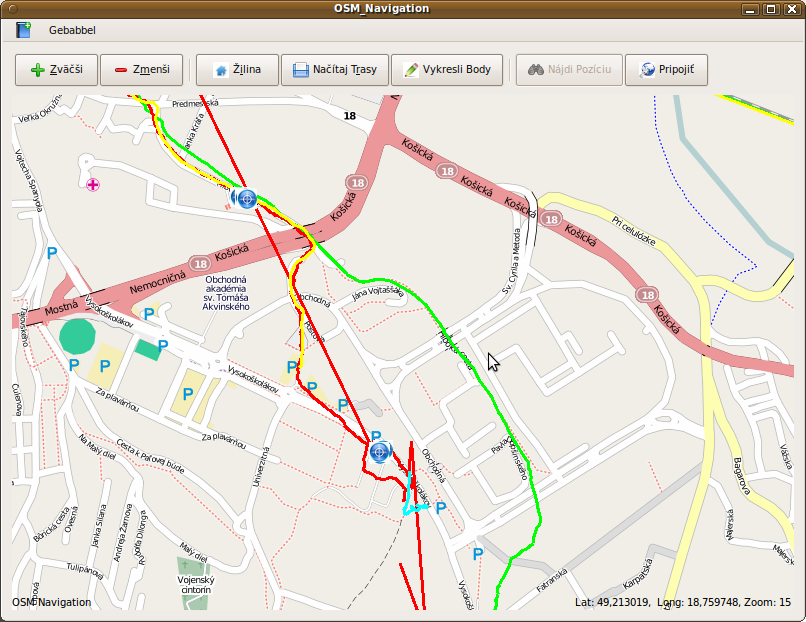
\includegraphics[width=14.5cm]{obr/mapa}
\caption{Trasa a významné body vykreslené na OSM mape}
\end{figure}



Pri zmenšení alebo zväčšení mapy musíme prekresliť na mape nové časti pretože pri priblížení alebo vzdialení sa nám mierkou zmenil obrázok na obrázok s iným detailom čo môžme spozorovať aj úplne iným snímkom.\\
Základné zmeny ktoré sa pri prekresľovaní dejú môžeme rozdeliť na dve časti: 
\begin{list}{•}
\item presúvanie sa po mape 
\item
\item zmena veľkosti mierky (`zoomovanie`)
\end{list}

\paragraph{Presúvanie sa po mape}
Program si pamätá jednu základnú súradnicu v jeho strede tzv. center. Od tejto súradnice sa odvíja celková poloha mapy ktorá je viditeľná.\\
Posun po mape je riešený dvoma spôsobmi:
\begin{list}{•}
\item posun klávesovými šípkami
\item
\item posun uchytením mapy myšou presun do žiadanej časti
\end{list}
Pri každej zmene mapy je potrebné v aplikačnej časti programu prepočítať nové hodnoty každej časti mapy. 


\paragraph{Zmena veľkosti mierky}
Ak chceme mapu zmenšiť, alebo zväčšiť môžeme tak urobiť viacerými spôsobmi:
\begin{list}{•}
\item dvojkliknutím na plochu mapy(ľavé tlačidlo priblíži mapu a pravé mapu vzdiali)
\item
\item rolovaním kolieskom myši 
\item kliknutím na tlačidlá priblíženia a vzdialenia
\end{list}
Pri týchto úkonoch sa vyvolávajú funkcie ktoré zmenia nastavenia priblíženia mapy (zoom-u) a následne sa vyvolá prekreslenie mapy.

\subsection{Pripojenie GPS zariadenia}
\paragraph{}
V tejto aplikácii existujú dve možnosti ako zariadenie pripojiť. Na výber nás v aplikácii vyzve podoknom (obr. 4.2). Prvá možnosť je pripojenie pomocou USB portu kde po pripojení vytvára OS port \textit{ttyUSB0}. Z tohto portu je možné čítať dáta vo forme NMEA protokolu. Druhou možnosťou je pripojiť zariadenie pomocou bezdrôtového pripojenia Bluetooth. V aplikácii je potrebné zadať MAC\footnote{\textbf{MAC} - Riadenie prístupu k médiu (Media Acces Control) = hardvérová adresa}. V prípade, že si v aplikácii zvolíme bezdrôtové pripojenie musíme zadať MAC adresu zariadenia (obr. 4.2). Po úspešnom pripojení už je možné čítať potrebné dáta.
\begin{figure}[ht]
\centering
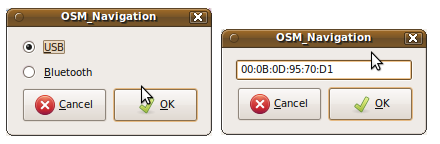
\includegraphics[width=12.5cm]{obr/volba_pris}
\caption{Výber spôsobu pripojenia}
\end{figure}


\subsection{Hľadanie aktuálnej pozície}
\paragraph{}
Hľadanie aktuálnej pozície má určitú postupnosť krokov. Ak je GPS zariadenie aktívne. Môže sa spustiť vyhľadávanie aktuálnej pozície. Príjem dát je riešený podprocesom ktorý spustí príkaz na čítanie dát z jedného z portu (USB – ttyUSB0, Bluetooth – rfcomm0).

Prístroj posiela dáta v protokole NMEA, dáta stačí rozdeliť a vhodne použiť na zistenie aktuálnej pozície. 

Po výzve používateľa sa výsledné dáta načítajú a pravidelne zobrazujú na mape. Vizuálnym výsledkom je mapa na ktorej je zobrazená naša aktuálna pozícia.
\begin{flushleft}
\textbf{Príkazy na čítanie dát:}
\begin{verbatim}
  cat /dev/rfcomm0  - v prípade pripojenia cez Bluetooth
  cat /dev/ttyUSB0  - v prípade zariadenia pripojeného cez USB
\end{verbatim}
\end{flushleft}

\section{Licencia aplikácie a požitých knižníc a programov}
\paragraph{}
V programe boli použité najme Knižnicou Qt , ktorá je pod licenciou GNU\footnote{\textbf{GNU} - } GPL~2\footnote{\textbf{GPL} - General public licence} pre nekomerčné využitie. 

Program Gebabbel má licenciu GNU GPL 2 a vlastník práv je Christoph Eckert. 
Program GPSbabel dovoľuje použitie pod licenciu GNU GPL 2, samotné časti programu môžu byť pod licenciu vlastníka samotnej časti.
